\section{Mapserver Peta Singapore}
 +\subsection{Cara Instalasi Mapserver}
 +\begin{enumerate}
 +\item
 +Download Mapserver atau disingkat MS4W di http://mapserver.org/download.html \ref{gambar1} seperti gambar dibawah ini
 +\begin{figure}[ht]
 +	    \centerline{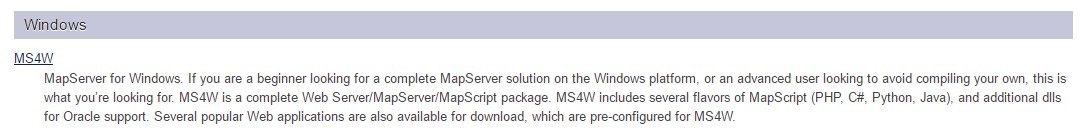
\includegraphics[width=0.50\textwidth]{figures/img1}}
 +	    \caption{Download MS4W}
 +		\label{gambar1}
 +		\end{figure}
 +\item
 +Setelah di download jalankan setupnya, disini saya menggunakan port 8080 karena port default 80 sudah dipakai oleh xampp \ref{gambar2} seperti gambar dibawah ini
 +\begin{figure}[ht]
 +	    \centerline{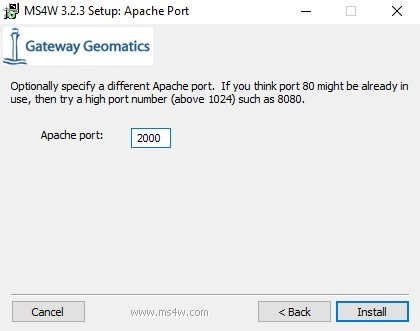
\includegraphics[width=0.50\textwidth]{figures/img2}}
 +	    \caption{Port 2000}
 +		\label{gambar2}
 +		\end{figure}
 +\item
 +Lalu tunggu instalasi sampai selesai \ref{gambar3} seperti gambar dibawah ini
 +\begin{figure}[ht]
 +	    \centerline{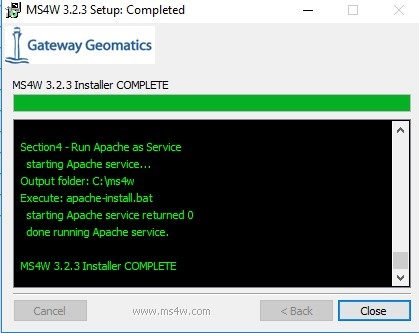
\includegraphics[width=0.50\textwidth]{figures/img3}}
 +	    \caption{Selesai}
 +		\label{gambar3}
 +		\end{figure}
 +\item
 +Setelah proses selesai silahkan buka browser favorit anda, kemudian ketikkan http://localhost:8080 di kotak isian URL.
 +\item
 +Jika anda melihat tampilan home MAPSERVER atau MS4W proses instalasi anda berhasil \ref{gambar4} seperti gambar dibawah ini
 +\begin{figure}[ht]
 +	    \centerline{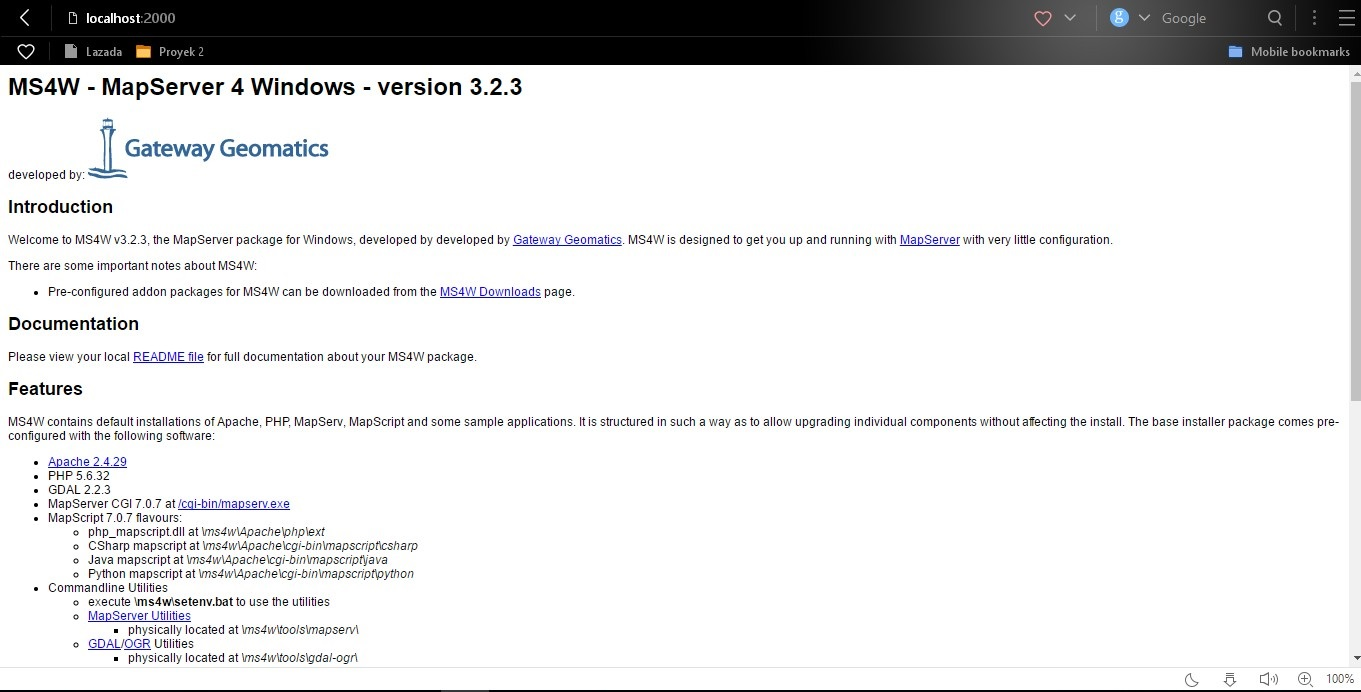
\includegraphics[width=0.50\textwidth]{figures/img4}}
 +	    \caption{Tampilan MS4W}
 +		\label{gambar4}
 +		\end{figure}
 +\end{enumerate}
 +Sekian Proses instalasi Mapserver pada Windows
